\chapter{Estado del arte}
\label{cap:estadoDeLaCuestion}


\section{¿Que es la Lectura Fácil?}
La Lectura Fácil (LF) es una forma de adaptar textos para una comprensión más sencilla del original. No se trata sólo de un resumen, sino de una simplificación del texto con un lenguaje, vocabulario, términos, oraciones, imágenes descriptivas y formato de forma simple, sencilla y adecuada para aquellas personas con discapacidad intelectual, con dificultad para el lenguaje, con alguna enfermedad y/o trastorno mental, en proceso de aprendizaje, etc. que, según estudios de la Unión Europea, alcanza al 30\% de la población.

El siguiente ejemplo muestra como es un texto de LF:


\begin{figure}[htb]
	\centering
	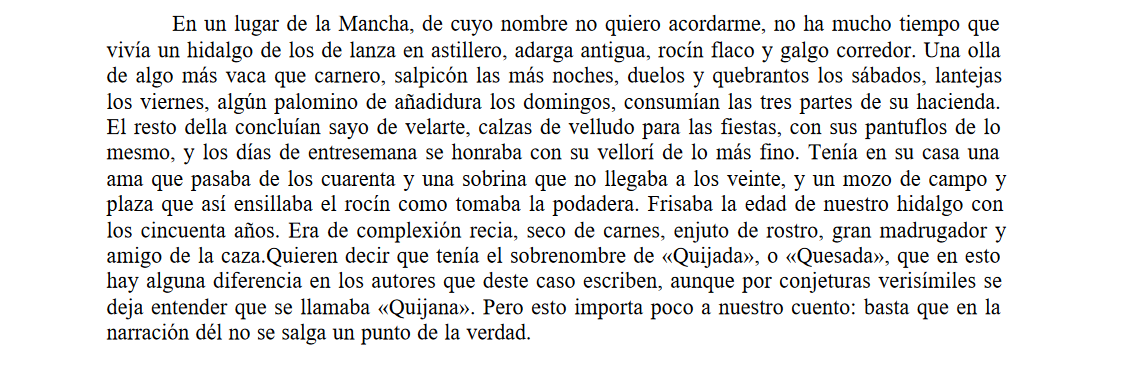
\includegraphics[width=1.15\textwidth]{Imagenes/Ejemplos/Cap1DonQuijote}
	\caption{Texto original de Don Quijote de la Mancha}
	\label{fig:Quijote}
\end{figure} 


\begin{figure}[htb]
	\centering
	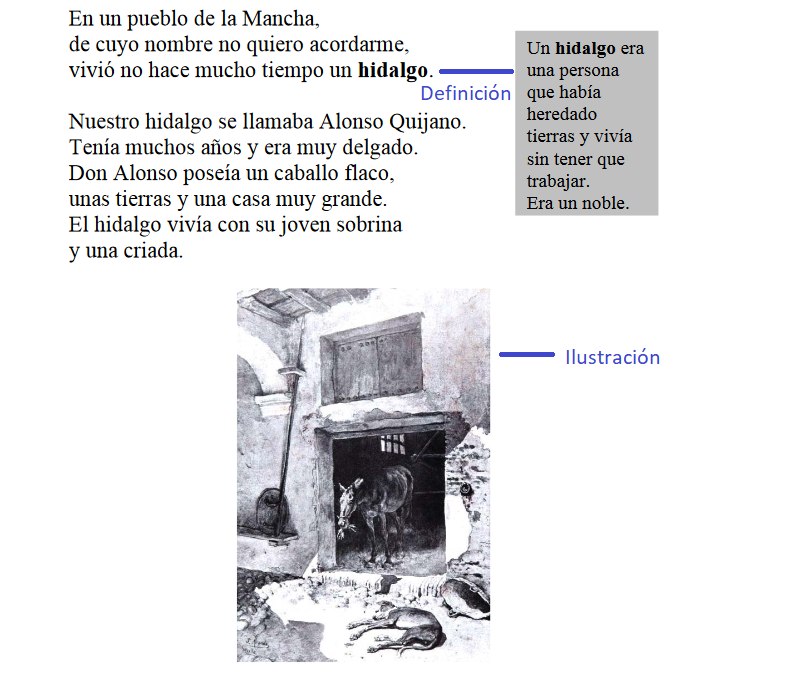
\includegraphics[width=0.7\textwidth]{Imagenes/Ejemplos/Cap1DonQuijoteLF}
	\caption{Texto LF de Don Quijote de la Mancha}
	\label{fig:QuijoteLF}
\end{figure}


\section{Un poco de Historia...}
El movimiento de la Lectura Fácil surgió en Suecia en 1968. En ese año se publicó el primer libro en Lectura Fácil y desde entonces hasta 1994 crearon 330 obras, entre 15 y 20 nuevas cada año.

Esto se extendió a los países vecinos de Noruega y Finlandia.

En Noruega, por ejemplo, la iniciativa se denomina \textit{Leser s$\emptyset$ker bok”}\footnote{\href{https://lesersokerbok.no/english/}{Leser s$\emptyset$ker bok}} (Lector busca libro) y es una alianza de 20 organizaciones, que incluyen editoriales y organizaciones de personas con discapacidad.

En 1988 se creó en Bruselas la organización \textit{Inclusion Europe}, la alianza europea de organizaciones que trabajan por los derechos de las personas con discapacidad, que actualmente agrupa a organizaciones y asociaciones de personas con discapacidad intelectual de 40 países europeos e Israel.

En 1998 se elaboró la guía \textit{«El camino más fácil: Directrices europeas para generar información de fácil lectura destinada a personas con discapacidad intelectual\footnote{\href{http://www.lecturafacil.net/media/resources/ILSMHcastell\%C3\%A0.pdf}{http://www.lecturafacil.net/media/resources/ILSMHcastell\%C3\%A0.pdf}}»} y se diseñó un logotipo europeo de Lectura Fácil, para identificar todos los textos redactados que siguieran sus pautas.

En España fue en 2003 cuando se creó la primera Asociación de Lectura Fácil en Barcelona. Desde entonces, surgen diversas organizaciones e iniciativas en pro de la Lectura Fácil por toda España.
\footnote{https://www.lecturafacilextremadura.es/historia/}

\section{¿Cómo se identifican los textos de Lectura Fácil?}
En los textos adaptados a Lectura Fácil vienen determinados por dos tipos de logotipos. En la figura \ref{fig:IFLA} es el logo que la Asociación de Lectura Fácil otorga a los textos que se adaptan a las normas de la Federación Internacional de Asociaciones de Bibliotecarios y Bibliotecas (IFLA), del inglés \textit{International Federation of Library Associations and Institutions}\footnote{\href{https://www.ifla.org/ES}{https://www.ifla.org/ES}}. Y la figura  \ref{fig:logoEuropeo}
Logo fomentado por Inclusion Europe \footnote{\href{http://www.inclusion-europe.eu/}{http://www.inclusion-europe.eu/}}.
\begin{figure}[htb]
\centering
	
\includegraphics[width=0.5\textwidth]{Imagenes/Logos/indice}
	\caption{Logo LF que cumplen las normas de la IFLA}
	\label{fig:IFLA}
\end{figure} 
\begin{figure}[htb]
	\centering
	
\includegraphics[width=0.3\textwidth]{Imagenes/Logos/indice2}
	\caption{Logotipo europeo de LF}
	\label{fig:logoEuropeo}
\end{figure} 
\section{Niveles de adaptación}
Es imposible adaptar un texto para todas las personas que necesiten este tipo de lectura.
 
La IFLA distingue entre los siguientes niveles de adaptación:
\begin{itemize}
	\item Primer nivel, es el más sencillo y simple con muchas imágenes y escaso texto, con una dificultas sintáctica baja.
\item Segundo nivel, es intermedio, menos sencillo que el anterior con un vocabulario y expresiones que son conocidas por todos, fácil de seguir y comprender e imágenes.
\item Tercer nivel, es el más complejo, con textos largos, palabras que no se conocen a menudo, con saltos en el tiempo y muy pocas imágenes. 
 \end{itemize}
\section{Pautas a seguir para la elaboración de Lectura Fácil}
 El primero documento de como elaborar texto adaptado a Lectura Fácil fue publicado por la IFLA. Hay otro que fue elaborado por varias organizaciones de Inclusion Europe bajo el título "Información para todos". 
 
 Las pautas que se deben seguir se vincula a la ortografía, gramática, léxico, estilo, diseño, imágenes, formato, etc. 
 
 Algunos ejemplos y recomendaciones son las siguientes:
 \begin{itemize}
 \item Uso de frases simples, cortas y con una estructura habitual.
 \item Uso de imágenes sencillas y pictogramas de apoyo al texto, de manera descriptiva.
 \item Cada frase debe ocupar una línea. Si no es fuese posible deberá ocupar varias líneas.
 \item Evitar oraciones impersonales y pasivas reflejas.
 \item Evitar el subjuntivo o la voz pasiva.
 \item Evitar signos ortográficos poco habituales. (%, &, / ...)
 \item Evitar abreviaturas, acrónimos y siglas
 \item Uso de palabras de uso cotidiano y evitar tecnicismos.
 \item Ideas principales
 \item Redactar en modo directo
 \item No dar conocimientos previos por conocidos.
 \item Evitar diseños cargados.
 \footnote{https://es.wikipedia.org/wiki/Lectura\_fácil\#Niveles} 
\end{itemize}
\section{Movimientos y asociaciones}
\begin{itemize}
	\item \href{https://www.lecturafacil.net/es/}{\textbf{Asociación de Lectura Fácil de Barcelona}}.
	
	 Es una entidad, creada en 2003, sin ánimo de lucro que trabaja para hacer accesible la lectura, la cultura y la información a todas las personas, con especial atención a aquellas con dificultades lectoras. 
	\item \href{https://www.lecturafacilextremadura.es/}{\textbf{Asociación Lectura Fácil Extremadura}}
	
	Organización sin ánimo de lucro que trabaja en pro de la promoción, implantación y difusión de la “Fácil Lectura”, encargada de  la generación de efectos de Accesibilidad, Inclusión, Integración, Participación Ciudadana y Realización Personal para distintos colectivos en situación de riesgo de exclusión económica y/o socio-cultural.
	\item \href{https://www.fundacionciudadania.es}{\textbf{Fundación Ciudadanía (Extremadura)}}.
	
	Organización sin ánimo de lucro, declarada de Utilidad Pública,de carácter social que realiza aportaciones y estrategias en el ámbito de la Innovación Educativa y el Empleo, extendiendo su ámbito de actuación a todo el territorio español, haciendo especial hincapié en Extremadura y en su vocación europea y latinoamericana.
	\item \href{https://odsextremadura.es/dilee-lectura-facil-extremadura/}{\textbf{Dilee Lectura Fácil (Extremadura)}}.
	
Empresa puntera en el territorio nacional y pionera dentro de la región extremeña, cuya misión principal es la implementación y consolidación de la Lectura Fácil en todos los ámbitos y sectores de la vida económica, socio-política, artística-cultural, educativa, y demás, de la comunidad extremeña.
	\item \href{https://www.lecturafacilmadrid.com/}{\textbf{Lectura Fácil Madrid}}.
	
	 Asociación constituida desde el año 2013 que tienen como objetivo  lograr que todas las personas puedan participar de forma activa y responsable en la sociedad y hacer realidad la democracia lectora. 
	\item \href{http://altavozcooperativa.org/}{\textbf{Cooperativa Altavoz (Madrid)}}.
	
	Cooperativa formada por personas con discapacidad
	que trabaja para mejorar la autonomía de todas las personas.
	
	\item \href{https://lecturafacileuskadi.net/}{\textbf{Lectura Fácil Euskadi (Bilbao)}}.
	
	Asociación que pretendde incentivar la creación, difusión y utilización de materiales en Lectura Fácil, a través de un programa de animación a la lectura dirigido a personas con dificultad en la comprensión lectora.
	\item \href{http://www.lecturafacyl.es/}{\textbf{Lectura Fácil Castilla y León (Palencia)}}.
	
	Entidad sin ánimo de lucro que trabaja para difundir la Lectura Fácil como herramienta de conocimiento entre las personas con dificultades de comprensión lectora en Castilla y León.
	\item \href{http://www.institutolecturafacil.org/}{\textbf{Instituto de Lectura Fácil (Sevilla)}}.
	
	Organización social con el objetivo de promover la accesibilidad cognitiva en España.
\end{itemize}

\section{Proyectos}
\begin{itemize}
\item \href{https://play.google.com/store/apps/details?id=org.changedyslexia.newdytective}{\textbf{Dytective para dislexia}}, aplicación gratuita, Dytective es la única herramienta científicamente validada que mejora las habilidades relacionadas con la lecto-escritura, para niños con o sin dificultades de lecto-escritura.
\item \href{https://www.lecturafacilextremadura.es/guia-en-lectura-facil-sobre-los-servicios-del-banco/}{\textbf{Guía en Lectura Fácil sobre los servicios del banco}}, Plena inclusión Galicia ha publicado una guía que trata sobre qué servicios te ofrece el banco y cómo manejar tu dinero. Esta guía esta en lectura fácil, es decir, que la guía es fácil de entender para personas con dificultades de comprensión.

\item \href{https://apkpure.com/es/l\%C3\%A9elo-f\%C3\%A1cil-educ-gallego/com.oneclick.ga.rayoluna}{\textbf{Léelo Fácil Educ. - Gallego}}, aplicación que sirve para leer un libro adaptado a lectura fácil
con dibujos, música y animaciones para que se entienda mejor.
\item
\href{https://plenainclusionmadrid.org/recursos/guia-de-uso-del-metro-de-madrid-en-lectura-facil/}{\textbf{Guía de uso del Metro de Madrid en Lectura fácil}}, en esta guía tiene como objetivo contribuir a que las personas con discapacidad intelectual puedan moverse por la red del suburbano de forma autónoma.
\item
\href{https://plenainclusionmadrid.org/noticias/el-museo-del-prado-guia-en-lectura-facil/}{\textbf{El Museo del Prado publica su primera guía en lectura fácil}}, el Museo del Prado ha publicado una guía en lectura fácil, que ofrece información sobre 10 obras maestras del museo. Realizada por el Museo en colaboración con Plena Inclusión Madrid.
\end{itemize}


%En el estado de la cuestión es donde aparecen gran parte de las referencias bibliográficas del trabajo. Una de las formas más cómodas de gestionar la bibliografía en {\LaTeX} es utilizando \textbf{bibtex}. Las entradas bibliográficas deben estar en un fichero con extensión \textit{.bib} (con esta plantilla se proporcionan 3, dos de los cuales están vacíos). Cada entrada bibliográfica tiene una clave que permite referenciarla desde cualquier parte del texto con los siguiente comandos:

%\begin{itemize}
%\item Referencia bibliografica con cite: \cite{ldesc2e}
%\item Referencia bibliográfica con citep: \citep{notsoshort}
%\item Referencia bibliográfica con citet: \citet{latexAPrimer}
%\end{itemize}

%Es posible citar más de una fuente, como por ejemplo %\citep{latexCompanion,LaTeXLamport,texKnuth}

%Después, latex se ocupa de rellenar la sección de bibliografía con las entradas \textbf{que hayan sido citadas} (es decir, no con todas las entradas que hay en el .bib, sino sólo con aquellas que se hayan citado en alguna parte del texto).

%Bibtex es un programa separado de latex, pdflatex o cualquier otra cosa que se use para compilar los .tex, de manera que para que se rellene correctamente la sección de bibliografía es necesario compilar primero el trabajo (a veces es necesario compilarlo dos veces), compilar después con bibtex, y volver a compilar otra vez el trabajo (de nuevo, puede ser necesario compilarlo dos veces). 
